\documentclass[../../main.tex]{subfiles}

\begin{document}

\subsection{Class diagram}

A UML class diagram describing the main entities involved in the system follows.

Farmers use the system to get weather information for their current location and to get advice on planting crops.
Farmers can also create discussion forums like a forum where they can upload their current problems in the system.

Telengana's policy makers have access to the farmer performance rankings in the DREAM system to distinguish between farmers who are performing well and those who are not.
The effectiveness of the policy is determined by comparing the ranking of the badly performing farmers over time.


Agronomists can answer farmers' questions and get the current weather data of the region and the best performing farmers in the system. They can also access local farmers according to the daily plan and update the daily plan daily.

\begin{figure}[H]
\centering
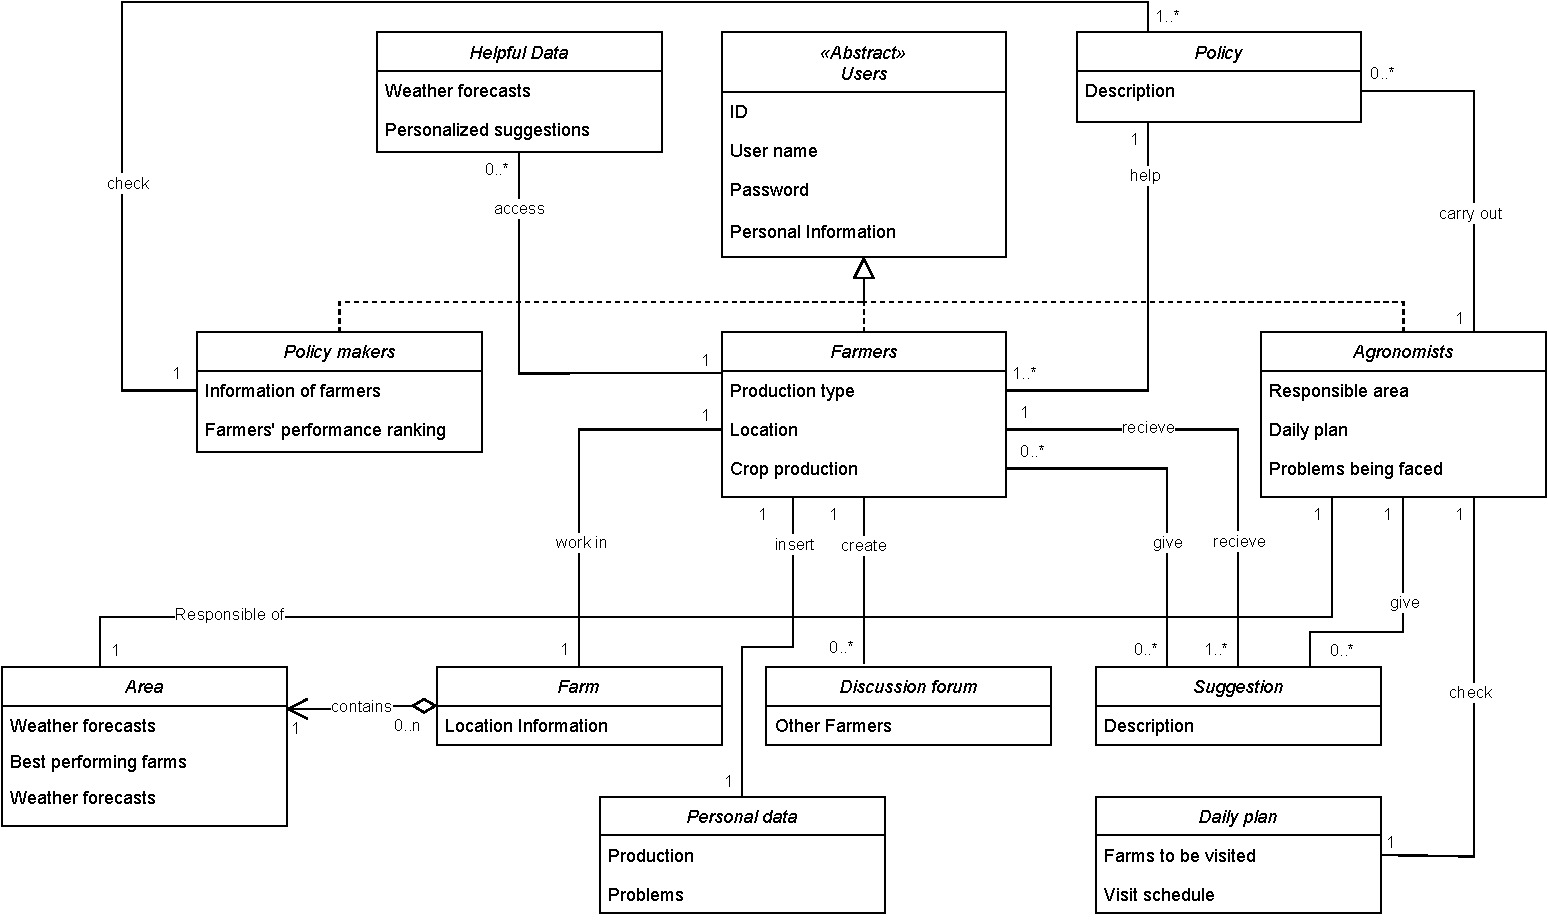
\includegraphics[width=5.55in, keepaspectratio]{RASD/image/class_diagram.pdf}
\caption{Class Diagram}
\end{figure}



\subsection{State chart diagrams}

The internal state of the main entities of the domain is better defined in the following UML
state diagrams.

\begin{figure}[H]
    \centering
    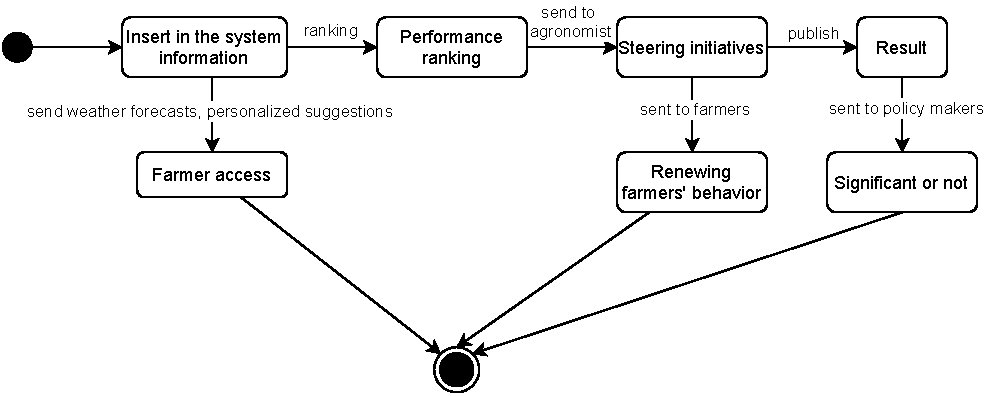
\includegraphics[width=\textwidth]{RASD/image/State_Chart.pdf}
    \caption{Statechart.}
\end{figure}

\subsection{Scenarios}

\newcounter{ScenarioCounter}

\stepcounter{ScenarioCounter}
\subsubsection{Giving special incentive to the performing well farmers.}

  Martini, a policy maker at Telengana, noticed that the weather conditions in the area where Farm A is located were not very good in recent days, with unstable temperatures, but Farm A had the highest production. After observing this phenomenon, he contacted Alex, the farmer in charge of Farm A, through the DREAM system, and rewarded him for being able to maintain high production despite the bad weather conditions, and encouraged Alex to share his farming experience.\\
  Alex is happy to receive the special incentives and share his experience to every farmer on the DREAM.


\stepcounter{ScenarioCounter}
\subsubsection{Helping farmer who needs help}

  Ann, also a policy maker at Telengana, noticed from the DREAM ranking table that the production of the farms managed by farmer Bob were far below the normal production. Noticing this phenomenon, she promptly contacted Bob and directed him to connect with the appropriate agronomists and quality farmers to provide him with technical guidance on planting the appropriate crops. At the same time, Ann added Bob to her watching list to monitor Bob's production in real time.\\
  Two months later, Bob's production were significantly higher than average.

\stepcounter{ScenarioCounter}
\subsubsection{Helping farmers to solve their problems}

  Mike owns a cornfield. In preparation for planting, Mike logged into his DREAM account, checked the weather information for his field, followed the system's recommendations for planting, and prepared the type of fertilizer that the system suggested. About a month after planting, Mike found that the corn in the field was not growing as expected. He opened DREAM and described his problem. Mike learned that the unsuitable humidity was causing the corn to grow too slowly, and he followed the advice in the forum to adjust the humidity of the land, and finally the corn grew at a normal rate.\\ 
  In the end he got more harvest than ever before.


\stepcounter{ScenarioCounter}
\subsubsection{Discussing with other farmers}

  Scarlett owned some fields, but she didn't know what kind of crops were appropriate to grow. She thought of DREAM, a software specifically for farmers, and that she might be able to get some useful information from the software. So she registered and logged into her DREAM account, opened the forum, shared information about the location of her farmland in the forum, and asked other farmers for their opinions. Soon there were many farmers sharing their experiences and opinions. Scarlett selected the opinions of most of these farmers and decided to grow soybeans on her own farm because they were best suited to the conditions of her field.

\stepcounter{ScenarioCounter}
\subsubsection{Agronomist supervision}

 Federico is a well-known agronomist who was invited to join the DREAM platform to help improve regional crop yields. One day he noticed that the eggplants planted by farmer Gary were rotting heavily, affecting the production of the farm. He looked at the weather conditions in Gary's area, the humidity of Gary's land and Gary's production information and discovered the problems Gary was having with the planting process. He reached out to Gary through the DREAM platform and instructed Gary to change his planting method.\\
Gary finally managed to save his eggplant field.

\end{document}
